\task{4.1}{Experiments with forward and backward Euler}
We solve
\[
u'=-50u,\qquad u(0)=1,\qquad 0\le t\le1.
\]
The exact solution is $u(t)=e^{-50t}$; in particular,
$u(1)=e^{-50}\simeq1.928749847963918\times10^{-22}$.

\partsol{a}
Forward Euler replaces the derivative by a forward difference:
\[
\frac{u^{n+1}-u^n}{\Delta t}=-50u^n
\quad\Longrightarrow\quad
\boxed{u^{n+1}=(1-50\Delta t)u^n.}
\]
To reach $t=1$ exactly, choose an integer $M$ and use $\Delta t=1/M$.
The following implementation is the recurrence used in the experiment:
\begin{lstlisting}[language=Python]
def forward_euler(M):
    dt = 1.0 / M
    u = 1.0
    for n in range(M):
        u = (1.0 - 50.0 * dt) * u
    return u
\end{lstlisting}
Since each step multiplies by the same factor $g=1-50\Delta t$, an independent formula is
$u^n=g^n$. This provides a direct check on the program.

\partsol{b}
Boundedness for arbitrarily many steps requires $|g|\le1$:
\[
-1\le1-50\Delta t\le1
\quad\Longrightarrow\quad
\boxed{0\le\Delta t\le0.04.}
\]
The numerical experiment compares steps on both sides of this limit. The final backward-Euler
column is discussed in part (d).
\begin{center}
\small
\begin{tabular}{rrrrr}
\toprule
$M$ & $\Delta t$ & $g_{\mathrm{FE}}$ & $u^M_{\mathrm{FE}}$ & $u^M_{\mathrm{BE}}$\\
\midrule
\tableinput{tables/task_4_1_stability.tex}
\bottomrule
\end{tabular}
\end{center}
For $\Delta t=0.05$, the factor is $-1.5$ and the magnitude grows. For
$\Delta t=1/24>0.04$, growth is slower but still present because $|g|>1$.
At the endpoint $\Delta t=0.04$, $g=-1$: the iterates alternate between $+1$ and $-1$.
They are bounded, so this endpoint is stable in the boundedness sense, but it does not reproduce
the physical decay. Strict decay requires $0<\Delta t<0.04$.
For $\Delta t=1/26$, the signs alternate while the magnitude decreases.
For $\Delta t=0.02$, $g=0$, so the numerical solution becomes zero after the first step.
That last fact is a property of this recurrence, not exact integration of the ODE.

\begin{figure}[H]
\centering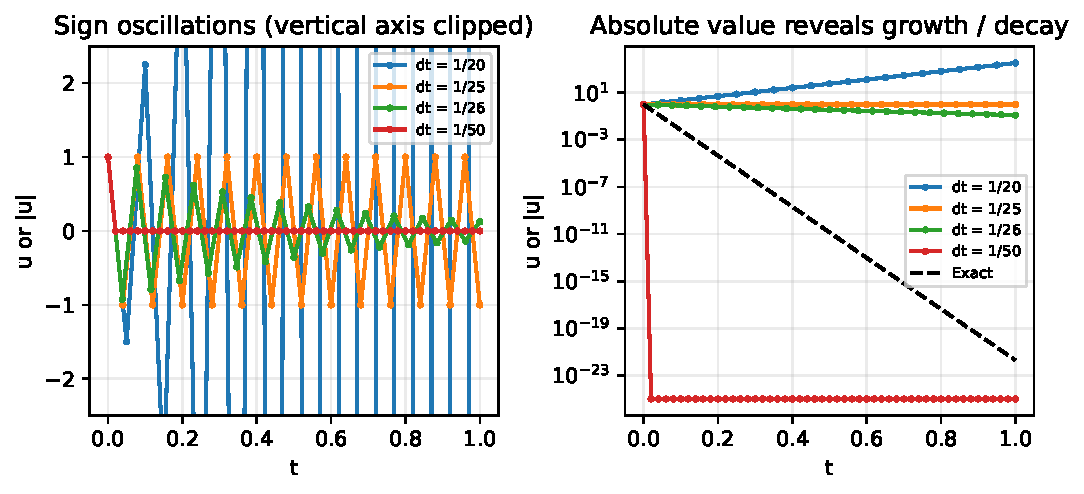
\includegraphics[width=\linewidth]{task_4_1_stability.pdf}
\caption{Forward Euler near its stability threshold. The left panel shows sign changes;
the logarithmic right panel shows whether their magnitudes grow or decay.}
\end{figure}
A finite observation interval alone cannot prove stability: a factor slightly larger than one
may not produce a spectacular blow-up by $t=1$. The recurrence and the bound on $|g|$ establish
the threshold exactly.

\partsol{c}
At the common final time $T=1$, define
\[
E(\Delta t)=\left|u^M-e^{-50}\right|,\qquad
p_{\mathrm{obs}}=\log_2\frac{E(\Delta t)}{E(\Delta t/2)}.
\]
We use sufficiently small steps to enter the asymptotic regime:
\begin{center}
\small
\begin{tabular}{rrrrr}
\toprule
$M$ & $\Delta t$ & $u^M$ & Absolute error & $p_{\mathrm{obs}}$\\
\midrule
\tableinput{tables/task_4_1.tex}
\bottomrule
\end{tabular}
\end{center}
The observed orders approach one. The very small absolute errors reflect the fact that the
exact final temperature is already about $10^{-22}$. They should be interpreted relative to
that final value, rather than as an indication that coarse steps are exceptionally accurate.

To explain why the fine steps in the table are useful, expand the logarithm for $50\Delta t<1$:
\begin{align*}
\log(1-50\Delta t)&=-50\Delta t-\frac{50^2}{2}\Delta t^2+O(\Delta t^3),\\
\log u^M&=\frac{1}{\Delta t}\log(1-50\Delta t)
=-50-1250\Delta t+O(\Delta t^2).
\end{align*}
Thus
\[
u^M=e^{-50}\bigl(1-1250\Delta t+O(\Delta t^2)\bigr),
\qquad
\boxed{E(\Delta t)=1250e^{-50}\Delta t+O(\Delta t^2).}
\]
The leading error is proportional to $\Delta t$. To see its asymptotic ratio clearly,
$1250\Delta t$ should be small, which is a stronger requirement than stability alone.
\begin{figure}[H]
\centering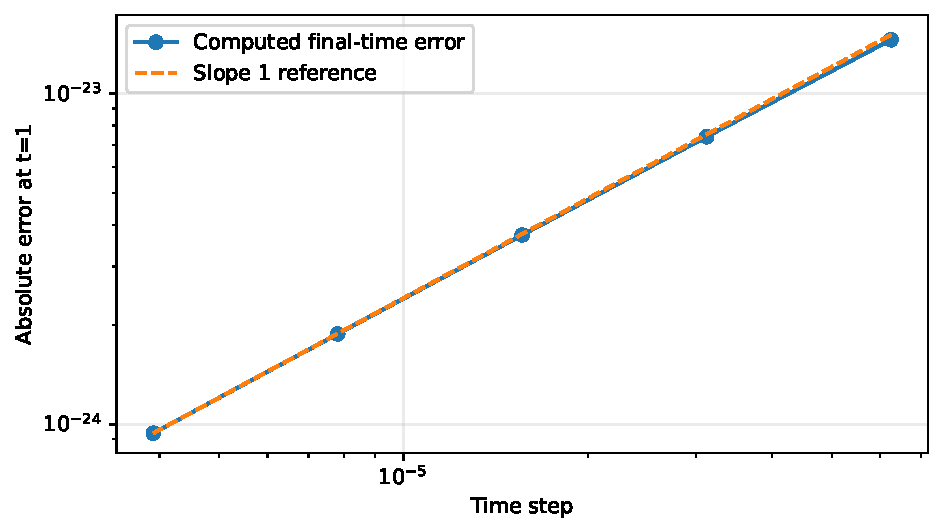
\includegraphics[width=.85\linewidth]{task_4_1_order.pdf}
\caption{Final-time forward-Euler error. The computed curve approaches the slope-one reference.}
\end{figure}

\partsol{d}
Backward Euler evaluates the right-hand side at the new time:
\[
\frac{u^{n+1}-u^n}{\Delta t}=-50u^{n+1}.
\]
Rearranging,
\[
(1+50\Delta t)u^{n+1}=u^n,
\qquad
\boxed{u^{n+1}=\frac{u^n}{1+50\Delta t}.}
\]
An implementation changes only the multiplication factor:
\begin{lstlisting}[language=Python]
def backward_euler(M):
    dt = 1.0 / M
    u = 1.0
    for n in range(M):
        u = u / (1.0 + 50.0 * dt)
    return u
\end{lstlisting}
For every $\Delta t>0$, $0<g_{\mathrm{BE}}=1/(1+50\Delta t)<1$.
Therefore the sequence stays positive and decreases, whatever the step size: there is
\emph{no finite upper stability limit}. The table includes steps larger than the forward-Euler
limit; they remain bounded with backward Euler.

Unconditional stability does not imply arbitrary accuracy. For example, taking one step with
$\Delta t=1$ gives $u^1=1/51\simeq0.01961$, far larger than $e^{-50}$.
Backward Euler is also first-order accurate; indeed,
\[
\log u^M=-\frac{1}{\Delta t}\log(1+50\Delta t)
=-50+1250\Delta t+O(\Delta t^2).
\]
It approaches the exact final value from above as the step is refined.

\task{5.1}{Warm-up: the one-dimensional heat equation}
Consider $u_t=\alpha u_{xx}$ for $0<x<L$ with prescribed boundary temperatures.
Let $x_i=i\Delta x$, where $\Delta x=L/N$.

\partsol{a}
Replace the spatial derivative while retaining continuous time. For $1\le i\le N-1$,
\[
\boxed{\frac{\dd u_i}{\dd t}
=\alpha\frac{u_{i+1}(t)-2u_i(t)+u_{i-1}(t)}{\Delta x^2}.}
\]
This is a system of $N-1$ ODEs. The boundary values $u_0(t)$ and $u_N(t)$ are known data;
they enter the equations adjacent to the boundaries.

\partsol{b}
Apply forward Euler to each ODE:
\[
\frac{u_i^{n+1}-u_i^n}{\Delta t}
=\alpha\frac{u_{i+1}^n-2u_i^n+u_{i-1}^n}{\Delta x^2}.
\]
Solving for the new value yields
\[
\boxed{u_i^{n+1}=u_i^n+
\frac{\alpha\Delta t}{\Delta x^2}
\bigl(u_{i+1}^n-2u_i^n+u_{i-1}^n\bigr).}
\]
Only level-$n$ values occur on the right, so every new interior value can be computed
independently once the old level is available.

\partsol{c}
The dimensionless combination is
\[
\boxed{r_x=\frac{\alpha\Delta t}{\Delta x^2}.}
\]
Its units cancel exactly as in Task 1.2(a), with $t$ replaced by $\Delta t$ and $L$ by
$\Delta x$. It compares the time step with the diffusion time $\Delta x^2/\alpha$
across a single grid cell. The update becomes
\[
u_i^{n+1}=(1-2r_x)u_i^n+r_xu_{i-1}^n+r_xu_{i+1}^n.
\]
Task 6.2 will show that this explicit scheme requires $r_x\le1/2$.

\task{5.2}{The two-dimensional update rule}
\partsol{a}
At an interior node the semi-discrete ODE is
\[
\frac{\dd u_{i,j}}{\dd t}
=\alpha\left[
\frac{u_{i+1,j}-2u_{i,j}+u_{i-1,j}}{\Delta x^2}
+\frac{u_{i,j+1}-2u_{i,j}+u_{i,j-1}}{\Delta y^2}\right].
\]
Define $r_x=\alpha\Delta t/\Delta x^2$ and $r_y=\alpha\Delta t/\Delta y^2$.
Applying forward Euler gives
\begin{align*}
\boxed{\begin{aligned}
u_{i,j}^{n+1}=u_{i,j}^n
&+r_x\bigl(u_{i+1,j}^n-2u_{i,j}^n+u_{i-1,j}^n\bigr)\\
&+r_y\bigl(u_{i,j+1}^n-2u_{i,j}^n+u_{i,j-1}^n\bigr).
\end{aligned}}
\end{align*}
The scheme is used at $1\le i\le N_x-1$, $1\le j\le N_y-1$.
Dirichlet boundary nodes are set to the prescribed data rather than updated by this formula.

\partsol{b}
For equal spacings $h$, let $r=\alpha\Delta t/h^2$. Then
\[
\boxed{u_{i,j}^{n+1}=u_{i,j}^n+r\left(
u_{i-1,j}^n+u_{i+1,j}^n+u_{i,j-1}^n+u_{i,j+1}^n-4u_{i,j}^n\right).}
\]
This is forward time, centred space (FTCS): forward Euler in time and central second
differences in space.

\partsol{c}
The space-time stencil has five inputs at level $n$ and one output at level $n+1$:
\[
\begin{array}{ccccc}
&&u^n_{i,j+1}&&\\[2pt]
&u^n_{i-1,j}&u^n_{i,j}&u^n_{i+1,j}&\\[2pt]
&&u^n_{i,j-1}&&
\end{array}
\quad\xrightarrow{\ \text{update}\ }\quad u^{n+1}_{i,j}.
\]
Their weights are $r$ at each neighbour and $1-4r$ at the old centre. There is no dependency
on another node at level $n+1$, and no diagonal input.

\partsol{d}
Fix the arithmetic order used by the supplied C++ implementation:
\begin{lstlisting}[language=C++]
sum = ((west + east) + south) + north;
next = centre + r * (sum - 4.0 * centre);
\end{lstlisting}
The operation count is
\begin{center}
\begin{tabular}{lr}
\toprule
Operation & Floating-point operations\\
\midrule
Sum four neighbours & 3 additions\\
Multiply centre by 4 & 1 multiplication\\
Subtract from neighbour sum & 1 subtraction\\
Multiply by $r$ & 1 multiplication\\
Add old centre & 1 addition\\
\midrule
Total & 7\\
\bottomrule
\end{tabular}
\end{center}
Index arithmetic and loop counters are integer operations and are excluded.
The parameter $r$ is computed once before the loop. Other algebraically equivalent expressions
can have different operation counts; all later cost estimates use this seven-operation convention.

Each update uses \textbf{five field values}: the old centre and four old neighbours, and writes
one new value. With doubles, the naive load/store count is $5\times8+8=48$ bytes per update.
This is an access count, not necessarily main-memory traffic: adjacent updates reuse values in
cache. With ideal reuse, old-array reads and new-array writes have a lower data-volume scale
of $16$ bytes per updated node, before effects such as write allocation. The low ratio of
arithmetic to data movement explains why stencil performance often depends strongly on memory bandwidth.

\task{5.3}{Interpreting the update}
\partsol{a}
Collect the old-centre terms in Task 5.2(b):
\[
\boxed{u^{n+1}_{i,j}=(1-4r)u^n_{i,j}
+r u^n_{i-1,j}+r u^n_{i+1,j}+r u^n_{i,j-1}+r u^n_{i,j+1}.}
\]
Thus $w_0=1-4r$ and each neighbour has weight $r$.
Their sum is
\[
(1-4r)+r+r+r+r=1.
\]
If every old value, including the boundary data read by the stencil, equals a constant $C$,
then the new value is $C$ times this sum, hence $C$. Uniform temperature is preserved exactly
in exact arithmetic. If an imposed boundary has a different value, the complete old field is
not uniform and diffusion should occur.

\partsol{b}
With $\bar u_4$ denoting the four-neighbour average,
\[
u^{n+1}_{i,j}-u^n_{i,j}=4r(\bar u_4-u^n_{i,j}).
\]
The centre moves towards its neighbours' average. A colder centre warms up, a hotter centre
cools down, and a balanced centre does not change at this step. For $0\le r\le1/4$, the
factor $4r$ lies in $[0,1]$: the new value is a genuine weighted average of old values.
At $r=1/4$, the old centre receives zero weight and the update equals the neighbour average.
For $r>1/4$, the centre weight becomes negative; Task 6.4 explains the resulting loss of
the maximum principle.

\task{5.4}{Insulated edges in two dimensions}
\partsol{a}
Suppose $x=0$ is insulated, so $u_x(0,y,t)=0$, and the other three edges are Dirichlet.
The nodes $(0,j)$ for $1\le j\le N_y-1$ now have unknown temperatures, in addition to the
ordinary interior nodes. The nodes on $x=L_x$, $y=0$, and $y=L_y$ remain prescribed.

Place a ghost column one step outside the left edge at $x_{-1}=-\Delta x$.
Approximate the boundary derivative by a centred difference:
\[
\frac{u^n_{1,j}-u^n_{-1,j}}{2\Delta x}=0
\quad\Longrightarrow\quad
\boxed{u^n_{-1,j}=u^n_{1,j}.}
\]
Refresh this relation before each time-step update. Applying the same heat stencil at $i=0$ gives
\[
\boxed{u^{n+1}_{0,j}=u^n_{0,j}
+2r_x(u^n_{1,j}-u^n_{0,j})
+r_y(u^n_{0,j+1}-2u^n_{0,j}+u^n_{0,j-1}).}
\]
The factor two in the normal direction comes from replacing the exterior ghost value by the
interior mirror value. The derivative is zero because the extension is symmetric across the wall.

\partsol{b}
\textbf{An insulated edge meeting a Dirichlet edge.}
The Dirichlet condition fixes the corner temperature. We impose that value and do not time-step
the corner as an unknown. For example, $(0,0)$ is fixed by the bottom edge even though it also
lies on the insulated left edge. Smooth solutions require compatible boundary data; if the data
are incompatible at the junction, local regularity can be reduced. This does not make it
appropriate to overwrite a prescribed Dirichlet corner using the evolution equation.

\textbf{Two insulated edges meeting.}
For a bottom-left insulated corner, both $u_x(0,0,t)=0$ and $u_y(0,0,t)=0$ hold, and the corner
is an unknown. Use the two mirror relations
\[
u_{-1,0}=u_{1,0},\qquad u_{0,-1}=u_{0,1}.
\]
Then
\[
\boxed{u^{n+1}_{0,0}=u^n_{0,0}
+2r_x(u^n_{1,0}-u^n_{0,0})+2r_y(u^n_{0,1}-u^n_{0,0}).}
\]
The diagonal ghost $( -1,-1)$ is unnecessary because the five-point stencil never reads it.
If an implementation stores it for convenience, double reflection gives $u_{-1,-1}=u_{1,1}$.

\partsol{c}
To avoid confusing a prescribed derivative with grid spacing, write the given condition as
$u_x(0,t)=H(t)$; this is the function called $h(t)$ in the question.
The centred derivative condition becomes
\[
\frac{u^n_1-u^n_{-1}}{2\Delta x}=H(t_n)
\quad\Longrightarrow\quad
\boxed{u^n_{-1}=u^n_1-2\Delta x\,H(t_n).}
\]
In 2D this applies separately for each boundary row, allowing $H=H(y_j,t_n)$.
The left-boundary second difference is therefore
\[
\frac{u_1-2u_0+u_{-1}}{\Delta x^2}
=\frac{2(u_1-u_0)}{\Delta x^2}-\frac{2H(t_n)}{\Delta x}.
\]
This provides the boundary evolution formula after multiplication by $\alpha\Delta t$.
The sign must be interpreted carefully: $u_x$ is a derivative in the positive $x$ direction.
On the left wall the outward normal is $(-1,0)$, so $\partial u/\partial n=-u_x$.
If a normal derivative $q_n$ is prescribed instead, then $H=-q_n$.
Fourier's physical heat flux also includes the conductivity and a minus sign.

\task{5.5}{Accuracy of the full scheme}
The task defines truncation error as a residual \emph{after division by the time step}:
\[
\tau^n_{i,j}=\frac{u(x_i,y_j,t_n+\Delta t)-u(x_i,y_j,t_n)}{\Delta t}
-\alpha\lap_hu(x_i,y_j,t_n),
\]
where the exact smooth solution is substituted.

\textbf{Step 1: expand the time quotient.}
\[
\frac{u(t+\Delta t)-u(t)}{\Delta t}
=u_t+\frac{\Delta t}{2}u_{tt}+O(\Delta t^2).
\]
\textbf{Step 2: expand the discrete spatial derivatives.}
Task 3.4 gives
\[
\lap_hu=u_{xx}+u_{yy}
+\frac{\Delta x^2}{12}u_{xxxx}
+\frac{\Delta y^2}{12}u_{yyyy}
+O(\Delta x^4+\Delta y^4).
\]
\textbf{Step 3: subtract and use the PDE.}
Because $u_t-\alpha(u_{xx}+u_{yy})=0$, the exact PDE terms cancel:
\[
\boxed{\tau=
\frac{\Delta t}{2}u_{tt}
-\frac{\alpha\Delta x^2}{12}u_{xxxx}
-\frac{\alpha\Delta y^2}{12}u_{yyyy}
+O(\Delta t^2+\Delta x^4+\Delta y^4).}
\]
Consequently,
\[
\boxed{\tau=O(\Delta t)+O(\Delta x^2)+O(\Delta y^2),\qquad p=1,\quad q=2.}
\]
The scheme is first order in time and second order in each spatial direction. It is consistent
because this residual tends to zero when all spacings tend to zero for a sufficiently smooth solution.

The undivided defect of one update is $\Delta t\,\tau$, with order
$O(\Delta t^2)+O(\Delta t\Delta x^2)+O(\Delta t\Delta y^2)$.
This explains why forward Euler's one-step local error can be called second order while the
time contribution to the PDE residual here is first order. They use different normalizations.
Consistency alone does not establish convergence; the stability restriction is derived next.
